  \documentclass[14pt, oneside]{book}
    \usepackage[margin=1in]{geometry} 
    \usepackage[brazilian]{babel}
    \usepackage{graphicx}
    \usepackage[utf8]{inputenc}
    \usepackage[T1]{fontenc}
    \usepackage{amsmath,amsthm,amssymb,amsfonts, mathtools}
    \usepackage{enumitem, verbatim, tikz, multicol}
    \usepackage{titlesec,hyperref, color, float, comment}
    
        \hypersetup{
            colorlinks=false, %set true if you want colored links
            linktoc=all,     %set to all if you want both sections and subsections linked
            linkcolor=blue,  %choose some color if you want links to stand out
        }
    \usepackage{listings}
    \titleformat{\chapter}[hang]{\bf\huge}{\thechapter}{2pc}{}
    \DeclarePairedDelimiter{\ceil}{\lceil}{\rceil}
    \date{\vspace{-5ex}}
    \lstset{language=Python}  
    \usepackage{pythonhighlight}
     
    \newcommand{\N}{\mathbb{N}}
    \newcommand{\Z}{\mathbb{Z}}
    \newcommand\tab[1][1cm]{\hspace*{#1}}
    \renewcommand{\qedsymbol}{$\blacksquare$}
     
    
\theoremstyle{definition}
    \newtheorem{problem}{Problema}
    \newtheorem{dica}{Dica}
    \newtheorem{gabarito}{Gabarito}
    \newtheorem{defn}{Definição}
    \newtheorem{teorema}{Teorema}
    
\begin{document}
    \pagenumbering{gobble}

    \begin{titlepage}
        \centering 
        
\includegraphics[scale = 0.8]{ufpe.png} \\
        \Large{\textbf{UNIVERSIDADE FEDERAL DE PERNAMBUCO}}\\
        \large{Departamento de Eletrônica e Sistemas}
        \vspace*{\stretch{2.0}}
   
        \Huge\textbf{Filtros RLC}\\
   
        \vspace*{\stretch{2.0}}
        \vfill
        \Large{Matheus Sobreira Farias}
        \\~\\
        \Large{Maio, 2019}
    \end{titlepage}

\addtocontents{toc}{\protect\hypertarget{toc}{}}
\tableofcontents
\mainmatter
        \chapter[Motivação]{\hyperlink{toc}{Motivação}}
            \tab O conceito de filtros mostra-se bastante importante na eletrônica como um todo, mas principalmente nas suas aplicações em comunicações. Ao longo da primeira unidade, estuda-se como projetar filtros Chebyshev e Butterworth passivos dadas suas especificações. \\
	        \tab No presente projeto, é pedido que se projete e simule 3 filtros, sendo 1 Chebyshev tipo I e os outros 2 sendo Butterworth, todos passivos:
            \begin{enumerate}
                \item Filtro Chebyshev tipo I passa alta com as seguintes especificações para a ordem mı́nima do filtro: Ripple na banda de passagem de $0,5$dB, $f_p = 4$kHz, $f_s = 2$kHz, $A_s = 60$dB e $R_L = 3$k$\Omega$.
                \item Filtro de Butterworth rejeita-faixa com as seguintes especificações para a ordem mı́nima do filtro: $Ap = 3$dB, $A_s = 60$dB, $B_p = 6$MHz, $B_s = 1, 5$MHz, $f_o = 25$MHz e $R_L = 1$k$\Omega$.
                \item Filtro de Butterworth passa-faixa com as seguintes especificações para a ordem mı́nima do filtro: $A_p= 1$dB, $A_s = 50$dB, $f_o = 500$kHz, $B_p = 4$KHz e $B_s =15$kHz.
            \end{enumerate}
           
             
            
        \chapter[Filtro Chebyshev I - passa alta]{\hyperlink{toc}{Filtro Chebyshev I - passa alta}}
            \tab Inicialmente calcula-se a ordem mínima do filtro usando a expressão \ref{ordemc}, onde $A_p$ é especificado no enunciado como $A_p =0.5$dB 
            \begin{equation}
            \label{ordemc}
            N = \left\lceil{\frac{\cosh^{-1}{(\sqrt{10^{A_s/10}-1}/\sqrt{10^{A_p/10}-1})}}{\cosh^{-1}{(\omega_p/\omega_s)}}}\right\rceil
            \end{equation}
            
            \begin{equation}
            \label{uhu}
            N = \ceil{6.57} = 7
            \end{equation}
            \tab De posse do valor de $N$, pode-se agora usar a tabela protótipo passa baixa com $A_p=0.5$dB, $\omega_p =1$rad/s e $R_s =0.5\Omega$\\
            \begin{figure}[H]
                \centering
                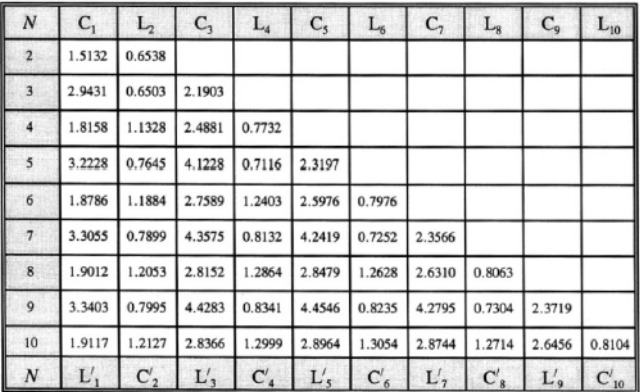
\includegraphics[scale=0.5]{tabelinha.jpeg}
                \caption{Tabela Protótipo Passa-Baixa}
                \label{a}
            \end{figure}\\~\\
            \tab Usando $R_S = R$ tem-se o circuito genérico da Figura \ref{circuitog}
            
            \begin{figure}[H]
                \centering
                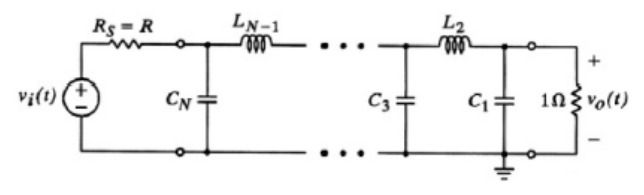
\includegraphics[scale=0.5]{circuitinho.jpeg}
                \caption{Circuito Genérico}
                \label{circuitog}
            \end{figure}
             
            \tab Com isso, temos:
             
            \begin{itemize}
                \item $R_S = 0.5\Omega$
                \item $R_L = 1\Omega$
                \item $C_1 = 3.3055$F
                \item $L_2 =0.7899$H
                \item $C_3 = 4.3575$F
                \item $L_4 = 0.8132$H
                \item $C_5 = 4.2419$F
                \item $L_6 = 0.7252$H
                \item $C_7 = 2.3566$F
            \end{itemize}\\
             
            \tab Como $f_p = 4k$Hz, então $k_f = 25132,7$, Como o filtro protótipo é passa-baixa, precisamos aplicar a transformação para o passa alta, substituindo os indutores por capacitores com capacitância $1/k_fL$ e os capacitores por indutores com indutância $1/k_fC$. Temos:
            
            \begin{itemize}
                \item $R_S = 0.5\Omega$
                \item $R_L = 1\Omega$
                \item $L_1 = 12.037\mu$H
                \item $C_2 =0.0505$mF
                \item $L_3 = 9.131\mu$H
                \item $C_4 = 48.928\mu$F
                \item $L_5 = 9.38\mu$H
                \item $C_6 = 0.055$mF
                \item $L_7 = 16.885\mu$H
            \end{itemize}\\
            
            \tab Como $R_L = 3k\Omega$, tem-se $k_i = 3000$. Para aplicar-se o escalonamento de impedância, multiplica-se o valor das resistências e das indutâncias por $k_i$, e divide-se as capacitâncias por $k_i$, logo, temos:
            
            \begin{itemize}
                \item $R_S = 1.5$k$\Omega$
                \item $R_L = 3$k$\Omega$
                \item $L_1 = 36.111$mH
                \item $C_2 =16.833$nF
                \item $L_3 = 27.393$mH
                \item $C_4 = 16.309$nF
                \item $L_5 = 28.140$mH
                \item $C_6 = 18.333$nF
                \item $L_7 = 50.655$mH
            \end{itemize}
            
            \tab Com a simulação abaixo é possível ver que próximo da frequência $f_p$ tem-se uma atenuação próxima de $-3.5$dB, considerando um possível erro devido às oscilações, e também para frequências abaixo de $f_p$ tem-se uma atenuação superior a $63.5$dB
            
            \begin{figure}[H]
                \centering
                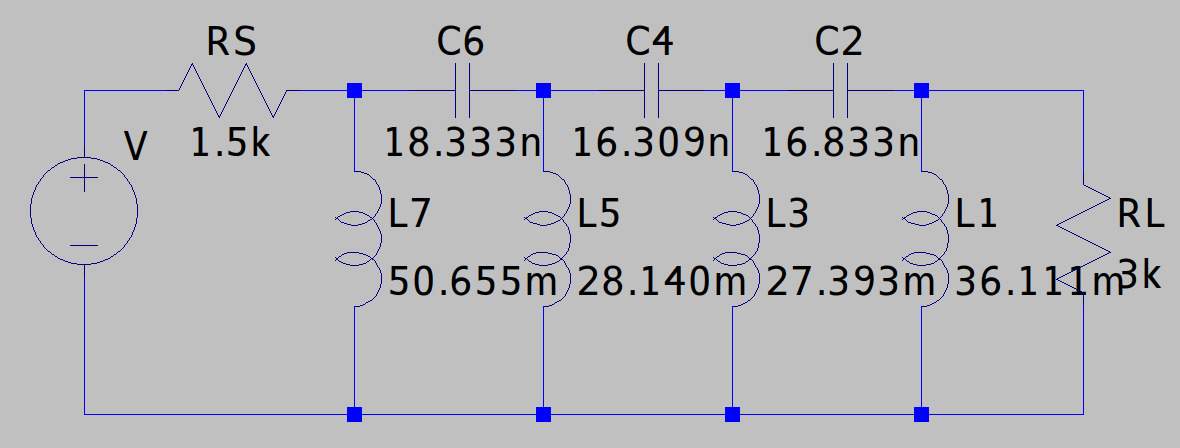
\includegraphics[scale=0.3]{circuitado.jpeg}
                \caption{Filtro Final}
                \label{a}
            \end{figure}
            
            \begin{figure}[H]
                \centering
                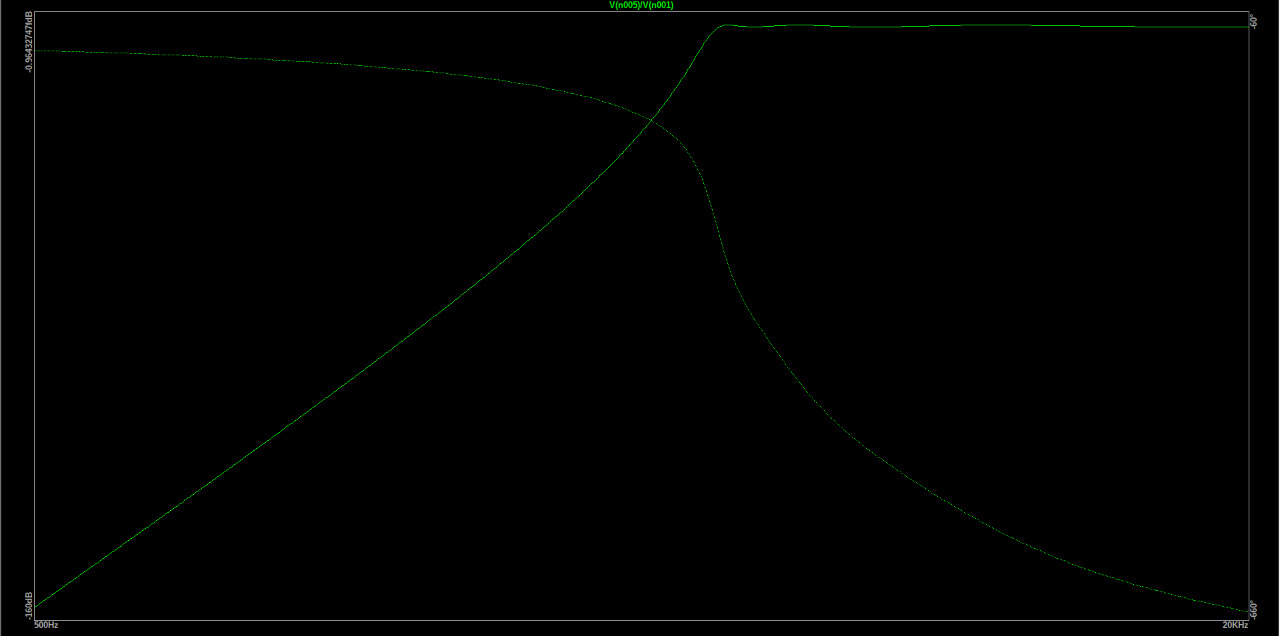
\includegraphics[scale=0.4]{bode.jpeg}
                \caption{Diagrama de Bode do Filtro}
                \label{a}
            \end{figure}
            
            \begin{figure}[H]
                \centering
                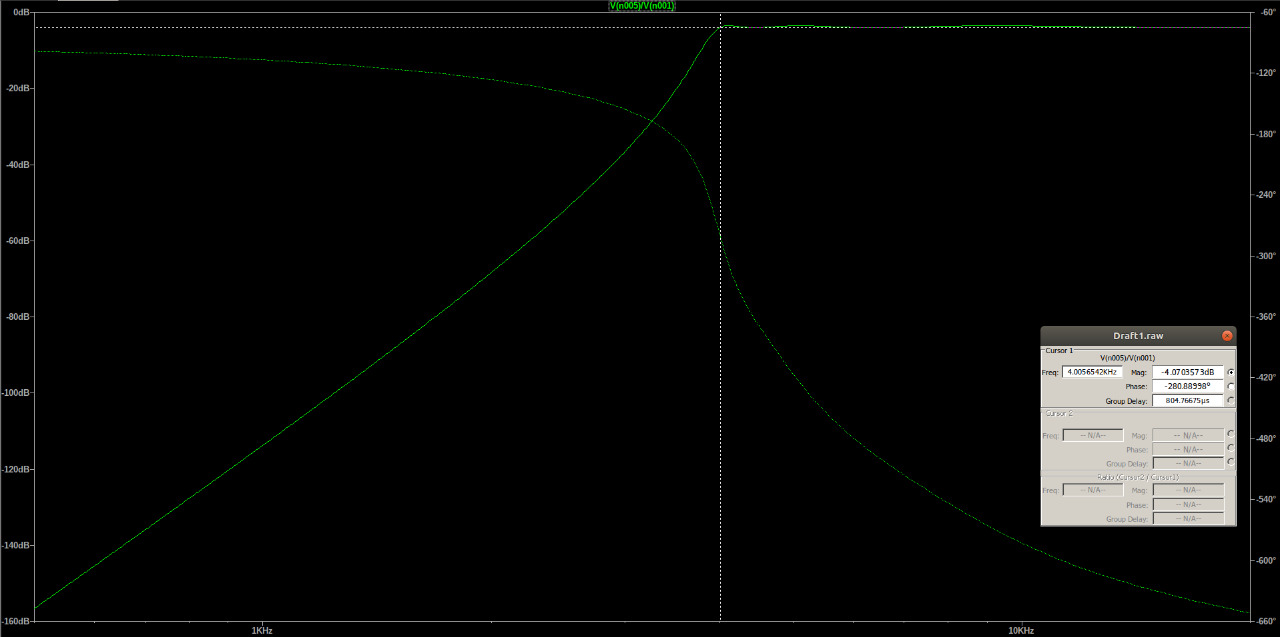
\includegraphics[scale=0.4]{fp.jpeg}
                \caption{Simulação próximo a $f_p$}
                \label{a}
            \end{figure}
            
            \begin{figure}[H]
                \centering
                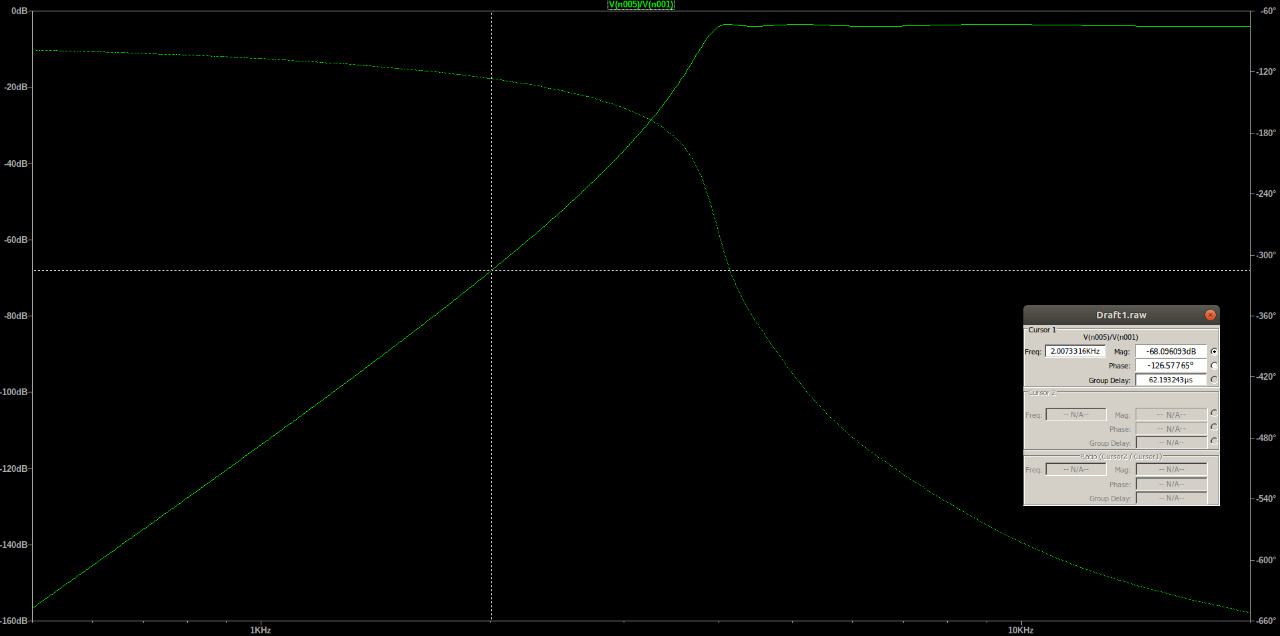
\includegraphics[scale=0.4]{fs.jpeg}
                \caption{Simulação próximo a $f_s$}
                \label{a}
            \end{figure}
            
            \begin{figure}[H]
                \centering
                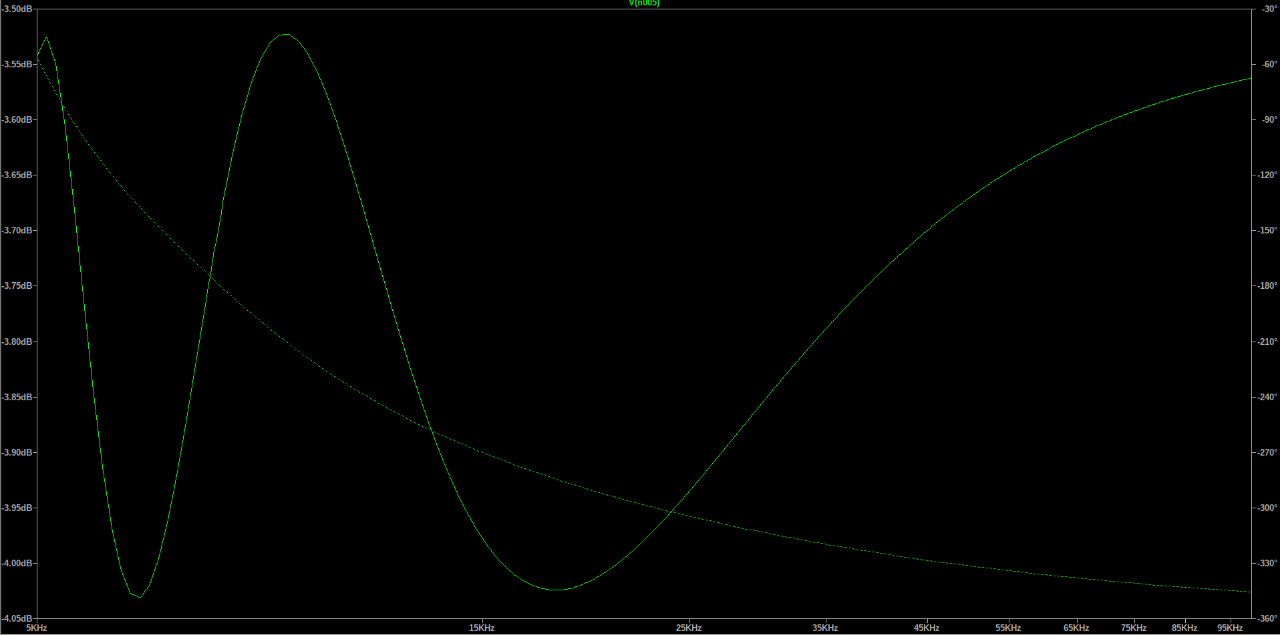
\includegraphics[scale=0.4]{ripple.jpeg}
                \caption{Ripple de 0.5}
                \label{a}
            \end{figure}
            
            
             
             
             
            
            \chapter[Filtro Butterworth - rejeita-faixa]{\hyperlink{toc}{Filtro Butterworth - rejeita-faixa}}
            
            \tab  Usando a equação \ref{ordembfa}:
              
            \begin{equation}
            \label{ordembfa}
            N = \left\lceil{\frac{{\log{(\sqrt{10^{A_s/10}-1}/\sqrt{10^{A_p/10}-1})}}}{{\log{(B_p/B_s)}}}}\right\rceil
            \end{equation}
            \begin{equation}
            N = \ceil{4,98} = 5
            \end{equation}
            Escolhe-se $R_S = R_L$.
            Temos:
            
            \begin{equation}
            |T(jw)|^2 = \frac{k^2}{1+w^{2N}}
            \end{equation}
            
            \begin{equation}
            |T(0)|^2 = k^2 = \frac{R_L}{R_L+R_S}=\frac{1}{4}
            \end{equation}
            
            \begin{equation}
            |A(jw)|^2 = \frac{w^{10}}{1+w^{10}}
            \end{equation}
            
            \begin{equation}
            A(s)A(-s) = \frac{s^5}{Q(s)}\cdot \frac{(-s)^5}{Q(-s)}
            \end{equation}
            
            Onde Q(s) é o polinômio de Butterworth de ordem 5
            \begin{equation}
            Q(s) = (s+1)(s^2+0.618s+1)(s^2+1.618s+1)
            \end{equation}
            
            \begin{equation}
            \label{eq}
            Z(jw) = \frac{1- A(jw)}{1+ A(jw)}
            \end{equation}
            
            Sabendo que cada termo da equação \ref{eq} representa uma admitância ou impedância, pode-se descobrir qual o valor da capacitância e da admitância, mas também pode-se usar a tabela \ref{tabelassa} para determinar tais componentes.
            
            \begin{figure}[H]
                \centering
                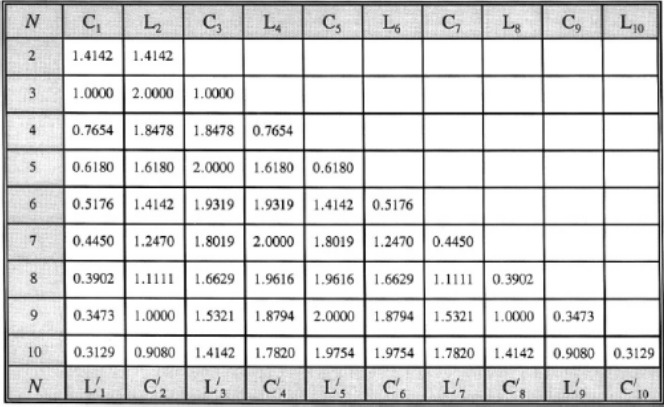
\includegraphics[scale=0.5]{tabelassa.jpeg}
                \caption{Tabela Protótipo Passa-Baixa}
                \label{tabelassa}
            \end{figure}
            
            Sendo assim, o circuito genérico é o mostrado na Figura \ref{circuitog}, logo, temos:
            
            \begin{itemize}
                \item $C_1= 0.618$F
                \item $L_2 = 1.618$H
                \item $C_3= 2$F
                \item $L_4 = 1.618$H
                \item $C_5 = 0.618$F
            \end{itemize}
            
            Como $w_0 = 157.08$Mrad/s e $B_p = 37,7$Mrad/s. Substitui-se cada indutor por um indutor de indutância:
            
            \begin{equation}
            B_pL/\omega_0^2
            \end{equation}
            
            Em paralelo com um capacitor de capacitância
            
            \begin{equation}
            1/(B_pL)
            \end{equation}
            
            E substitui-se cada capacitor por um indutor com indutância
            \begin{equation}
            1/(B_pC)
            \end{equation}
            
            Em série com capacitor de capacitância
            \begin{equation}
            B_pC/\omega_0^2
            \end{equation}
            Então tem-se, escalonado com $k_i = 3000$:
            \begin{itemize}
                \item $R_L = 3$k$\Omega$
                \item $R_S = 3$k$\Omega$
                \item $C_1= 0.15$pF
                \item $L_1 = 270\mu$H
                \item $C_2= 0.1\mu$F
                \item $L_2 = 393.4$nH
                \item $C_3= 0.48$pF
                \item $L_3 = 83\mu$H
                \item $C_4= 103$pF
                \item $L_4 = 393.4$nH
                \item $C_5= 0.15$pF
                \item $L_5 = 270\mu0$H
            \end{itemize}
            
            Tem-se o circuito final:
            
            \begin{figure}[H]
                \centering
                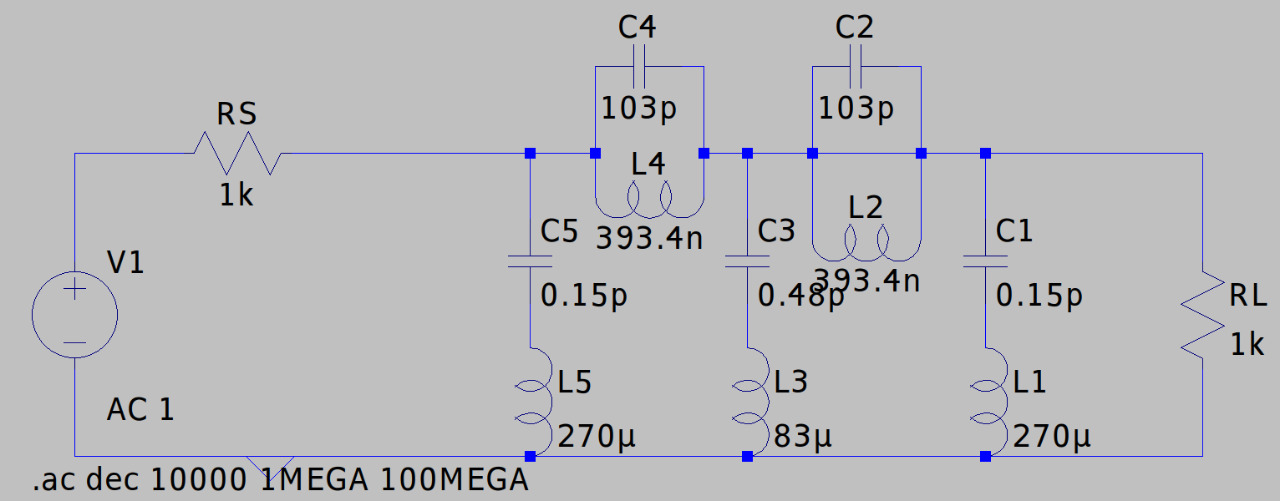
\includegraphics[scale=0.4]{rejeitacirc.jpeg}
                \caption{Circuito rejeita-faixa}
            \end{figure}
            
            \begin{figure}[H]
                \centering
                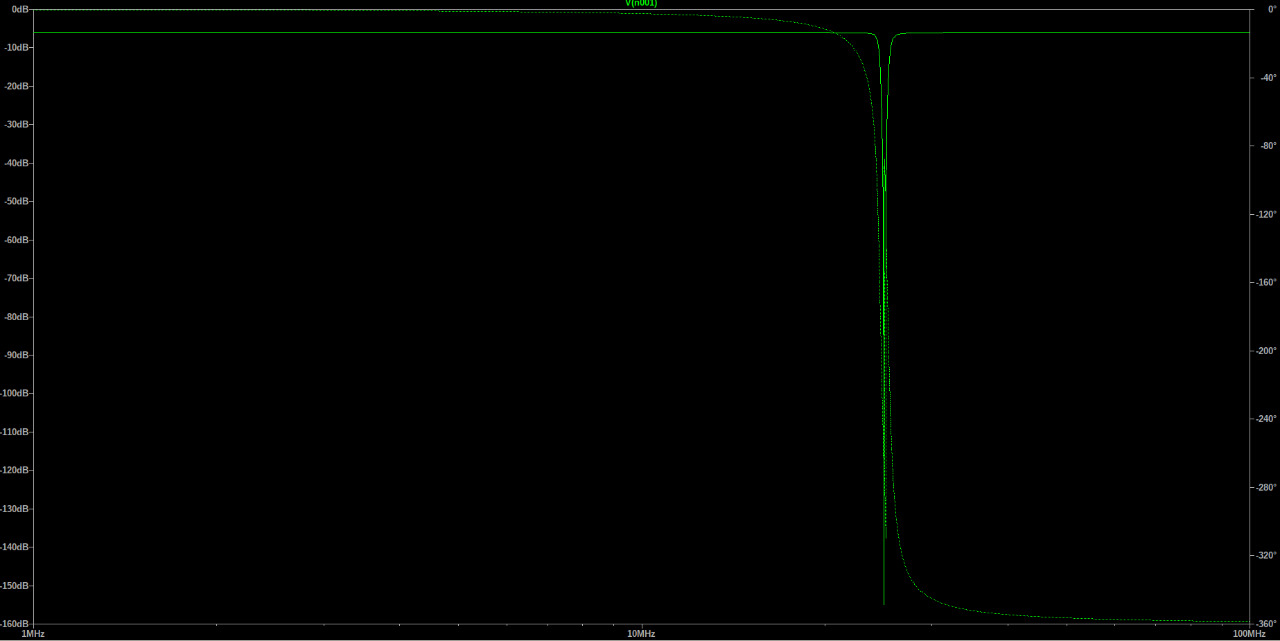
\includegraphics[scale=0.4]{rejeitando.jpeg}
                \caption{Filtro rejeita-faixa}
            \end{figure}
            
            \begin{figure}[H]
                \centering
                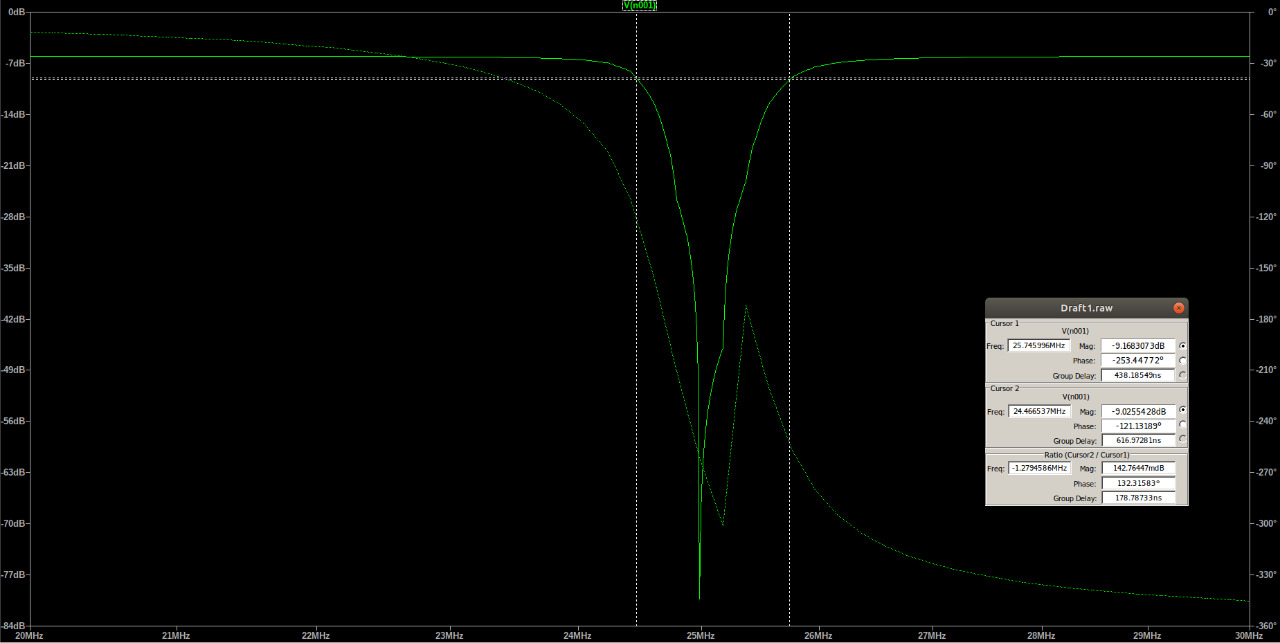
\includegraphics[scale=0.4]{rejeitamedida.jpeg}
                \caption{Simulação para ver $f_0$}
                \label{here}
            \end{figure}
            
            
            Pela Figura \ref{here}, pode-se ver que $f_0$ = $\sqrt{24.46\cdot 25.74} = 25.09$MHz. E a diferença entre as frequências $B_p = 0.63$MHz
            
            
            
            
            
                    
                
            \chapter[Filtro de Butterworth passa-faixa]{\hyperlink{toc}{Filtro de Butterworth passa-faixa}}
            
            \begin{equation}
            \label{ordembf}
            N = \left\lceil{\frac{{\log{(\sqrt{10^{A_s/10}-1}/\sqrt{10^{A_p/10}-1})}}}{{\log{(B_s/B_p)}}}}\right\rceil
            \end{equation}
                
            \begin{equation}
            N = \ceil{4,86} = 5
            \end{equation}
            Temos:
            
            \begin{equation}
            |T(jw)|^2 = \frac{k^2}{1+w^{2N}}
            \end{equation}
            
            \begin{equation}
            |T(0)|^2 = k^2 = \frac{R_L}{R_L+R_S}=\frac{1}{4}
            \end{equation}
            
            \begin{equation}
            |A(jw)|^2 = \frac{w^{10}}{1+w^{10}}
            \end{equation}
            
            \begin{equation}
            A(s)A(-s) = \frac{s^5}{Q(s)}\cdot \frac{(-s)^5}{Q(-s)}
            \end{equation}
            
            Onde Q(s) é o polinômio de Butterworth de ordem 5
            \begin{equation}
            Q(s) = (s+1)(s^2+0.618s+1)(s^2+1.618s+1)
            \end{equation}
            
            \begin{equation}
            Z(jw) = \frac{1- A(jw)}{1+ A(jw)}
            \label{op}
            \end{equation}
            
            
            Como já dito no rejeita-faixa, sabendo que cada termo da equação \ref{op} representa uma admitância ou impedância, podemos descobrir qual o valor da capacitância e da admitância, mas também pode-se usar a tabela \ref{tabelassa} para determinar tais componentes.
        
            
            Sendo assim, o circuito genérico é o representado na Figura \ref{circuitog}
            
            Logo, temos:
            
            \begin{itemize}
                \item $C_1= 0.618$F
                \item $L_2 = 1.618$H
                \item $C_3= 2$F
                \item $L_4 = 1.618$H
                \item $C_5 = 0.618$F
            \end{itemize}
            
            Para transformação em frequência:
            \begin{equation}
            \Omega = \frac{\omega^2-\omega_0^2}{B_p\omega}
            \end{equation}
            
            Usando $\omega_c = 1$ e $\omega_p = \Omega$:
            
            \begin{equation}
            \Omega = (10^{A_p/10}-1)^{1/2N}
            \end{equation}
            Temos:
            \begin{equation}
            \Omega = 1.144
            \end{equation}
            \begin{equation}
            B_{p(3dB)} = 1.144B_p
            \end{equation}
            
            Sendo assim, tem-se $\omega_0 =3,14$Mrad/s e $B_{p(3dB)} = 28.75$krad/s
            Substitui-se cada indutor por um indutor de indutância:
            
            \begin{equation}
            L/B_{p(3dB)}
            \end{equation}
            
            Em série com um capacitor de capacitância
            
            \begin{equation}
            B_{p(dB)}/(L\omega_0^2)
            \end{equation}
            
            E substitui-se cada capacitor por um indutor com indutância
            \begin{equation}
            B_{p(3dB)}/(C\omega_0^2)
            \end{equation}
            
            Em paralelo com capacitor de capacitância
            \begin{equation}
            C/B_{p(3dB)}
            \end{equation}
            Então temos, escalonado com $k_i = 1000$:
            \begin{itemize}
                \item $R_S = 1$k$\Omega$
                \item $R_L = 1$k$\Omega$
                \item $L_1 = 4.7\mu$H
                \item $C_1 =21.5$nF
                \item $L_2= 56.25$mH
                \item $C_2 = 1.8$pF
                \item $L_3= 1.45\mu$H
                \item $C_3 = 69.5$nF
                \item $L_4= 56.25$mH
                \item $C_4 = 1.8p$pF
                \item $L_5= 4.7\mu$H
                \item $C_5 = 21.5$nF
            \end{itemize}
            
            Tem-se o circuito final:
            
            \begin{figure}[H]
                \centering
                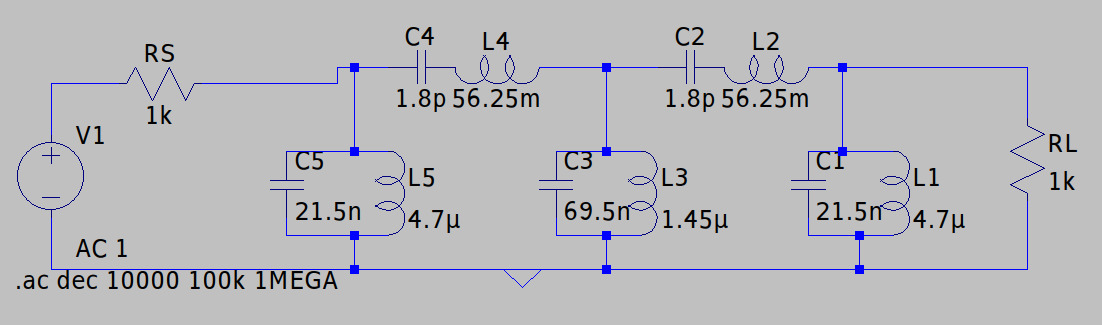
\includegraphics[scale=0.4]{FINAL.jpeg}
                \caption{Circuito passa-faixa}
            \end{figure}
            
            \begin{figure}[H]
                \centering
                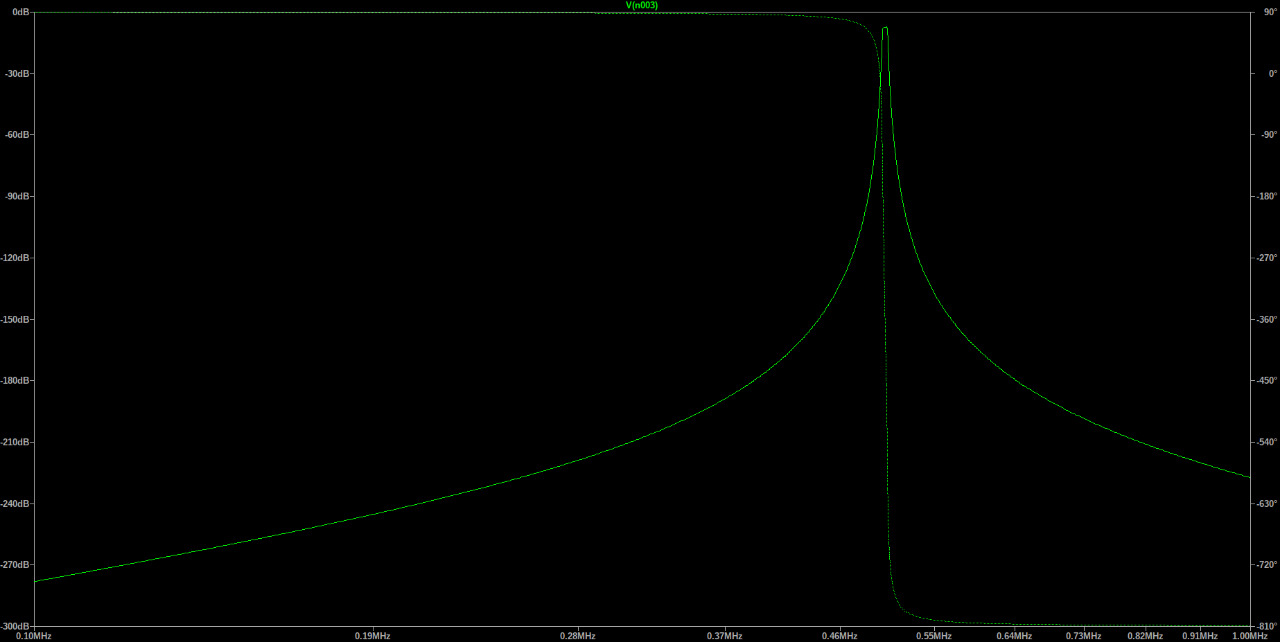
\includegraphics[scale=0.4]{passando.jpeg}
                \caption{Filtro passa-faixa}
            \end{figure}
            
            \begin{figure}[H]
                \centering
                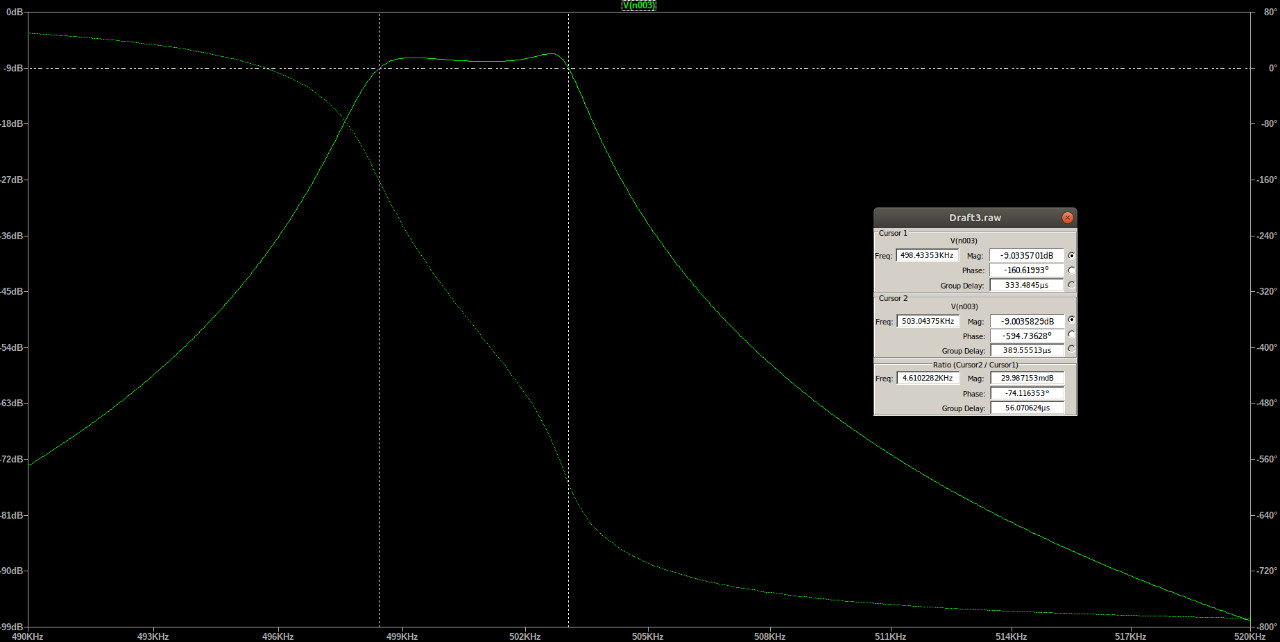
\includegraphics[scale=0.4]{PASSAMEDIDA.jpeg}
                \caption{Simulação para ver as frequências de corte}
                \label{fdown1}
            \end{figure}
            
            Pela Figura \ref{fdown1}, pode-se ver que $f_0 = \sqrt{498.43\cdot503.04 }$ = 500.7kHz. E a diferença entre as frequências $B_{p(3dB)}=4.97$kHz foi bem próximo do esperado.
                 
             
        \chapter[Conclusão]{\hyperlink{toc}{Conclusão}}
            \tab Por fim, foi possível aproveitar com este projeto a consolidação do aprendizado de projetos de filtros analógicos, os resultados couberam dentro de uma faixa de aceitação razoável, sujeito a pequenos erros de aproximação de cálculo.

\end{document}